\section{Application to carpentry and joinery accidents in EPICEA}
\label{sec:chap4_application_carpentry}

In this section, we consider the application of the proposed framework to occupational accident narratives from the French EPICEA database. We first describe the data and the construction of the study population. We then present the semantic factors identified within the four accident-process roles and assess their robustness. Finally, the Bayesian-network and recurrent-scenario results are presented.

\subsection{Corpus definition and study population}
\label{sec:chap4_carpentry_corpus}

The application was conducted on occupational accident narratives from the
construction sector of the EPICEA database. This sector covers heterogeneous
occupational activities involving different work situations, equipment, and
exposure conditions. Because the objective is to identify recurrent accident
processes that remain interpretable from a prevention perspective, the analysis
was conducted within a more occupationally coherent population. The available
company activity information was therefore used to define the study population
independently of the subsequent semantic factor discovery, Bayesian-network,
and recurrent-scenario analyses.

Carpentry and joinery was retained as a sufficiently represented and
occupationally specific activity group. The resulting corpus contains
417 accident narratives, corresponding to approximately 6.9\% of the
6,040 construction-sector accidents available in EPICEA. The purpose of this
restriction is not to obtain a representative subsample of the entire
construction sector, but to investigate recurrent accident processes within
a more coherent occupational setting.

Table~\ref{tab:chap4_carpentry_corpus_summary} summarizes the role-specific
corpora obtained from these narratives. Factual units constitute the
observations used for semantic factor discovery, whereas accident narratives
remain the resampling units for robustness assessment and the statistical
units used in the subsequent accident-level analyses.

\begin{table}[!htbp]
\centering
\footnotesize
\caption{Characteristics of the role-specific corpora for the carpentry and
joinery study population.}
\label{tab:chap4_carpentry_corpus_summary}
\renewcommand{\arraystretch}{1.15}
\setlength{\tabcolsep}{8pt}

\begin{tabular}{lccc}
\toprule
\textbf{Role}
& \textbf{Factual units}
& \textbf{Contributing accidents}
& \textbf{Mean units per contributing accident} \\
\midrule
A0 & 1,813 & 380 & 4.77 \\
A1 & 373   & 208 & 1.79 \\
B  & 549   & 338 & 1.62 \\
C  & 479   & 391 & 1.23 \\
\bottomrule
\end{tabular}
\end{table}

The amount of information available differs substantially across
accident-process roles. Work-context information is particularly detailed,
with multiple A0 units frequently extracted from the same narrative.
By contrast, explicit adverse-condition information is identified in only
about half of the accidents. Event/deviation information is available for
approximately four out of five accidents, while consequence information is
identified in almost all narratives.

These differences define distinct empirical conditions for semantic factor
discovery across the four roles. In particular, A0 is characterized by a
larger and denser semantic corpus, whereas A1 is based on substantially fewer
observations. The role-specific corpora should nevertheless not be interpreted
as separate accident populations: they are overlapping subsets of the same
417 narratives, since a single accident may contribute factual units to
several roles.

\subsection{Selection of role-specific semantic partitions}
\label{sec:chap4_carpentry_partition_selection}

Factual units were represented using the pretrained
Qwen3-Embedding-0.6B encoder \citep{zhang2025qwen3embedding}, without
task-specific fine-tuning. The UMAP--HDBSCAN configuration search was
conducted independently for each accident-process role using the search domain
reported in Table~\ref{tab:chap4_carpentry_search_domain}. The Cartesian
product of the varying parameters resulted in 120 candidate configurations per
role.

\begin{table}[!htbp]
\centering
\footnotesize
\caption{UMAP--HDBSCAN search domain used for semantic factor discovery in
the carpentry and joinery application.}
\label{tab:chap4_carpentry_search_domain}
\renewcommand{\arraystretch}{1.15}
\setlength{\tabcolsep}{6pt}

\begin{tabularx}{0.90\textwidth}{
>{\raggedright\arraybackslash}p{0.30\textwidth}
>{\raggedright\arraybackslash}X}
\toprule
\textbf{Parameter} & \textbf{Values} \\
\midrule
UMAP neighbourhood size & 5, 10, 20, 40, 80 \\
UMAP reduced dimension & 5, 10, 15 \\
UMAP minimum distance & 0 \\
UMAP input metric & cosine \\
HDBSCAN minimum cluster size & 8, 15, 25, 50 \\
HDBSCAN minimum samples & 5, 10 \\
HDBSCAN extraction rule & leaf \\
HDBSCAN distance metric & Euclidean \\
\bottomrule
\end{tabularx}
\end{table}

Figure~\ref{fig:chap4_carpentry_stability_landscape} shows the resulting
DBCV--reproducibility landscapes and the corresponding Pareto fronts. The
shape of these fronts differs substantially across roles. For A0, increasing
density-based separation is accompanied by a progressive decrease in
resampling reproducibility, producing a broad set of competing solutions.
A similar trade-off is observed for A1, although a smaller subset of
configurations occupies the most favourable part of the search space.

The B and C roles exhibit different patterns. For B, two Pareto-supported
configurations achieve substantially higher reproducibility than the remaining
candidate on the front while retaining similar DBCV values. For C, a distinct
group of configurations combines high reproducibility with comparatively high
DBCV, indicating a more consistently defined semantic structure than for the
upstream roles.

\begin{figure}[!htbp]
    \centering
    \includegraphics[width=\textwidth]
    {figs_ch4/stability_landscape_all_roles.png}
    \caption{DBCV and accident-resampling reproducibility for the
    UMAP--HDBSCAN configurations evaluated within each accident-process role.
    Grey points represent candidate configurations, blue points identify the
    Pareto front, and the red star indicates the configuration ultimately
    retained for each role.}
    \label{fig:chap4_carpentry_stability_landscape}
\end{figure}

The normalized Pareto fronts used for the final compromise selection are shown
in Figure~\ref{fig:chap4_carpentry_tchebycheff}. The selected A0 configuration
occupies an intermediate position between solutions favouring reproducibility
and those favouring density-based separation. For A1, the selected solution
retains high relative performance on both criteria and lies close to the
balanced region of the normalized front. For B, the selected configuration
preserves the high reproducibility of the best-performing solutions, whereas
the configuration providing the highest DBCV entails a marked loss of
reproducibility. The selected C configuration similarly represents an
intermediate compromise within a front whose solutions are all highly
reproducible.

\begin{figure}[!htbp]
    \centering
    \includegraphics[width=\textwidth]
    {figs_ch4/pareto_normalized_tchebycheff_all_roles.png}
    \caption{Normalized Pareto fronts used for final configuration selection.
    The cross indicates the ideal point, blue points represent Pareto-supported
    configurations, and red stars identify the configurations selected by the
    normalized Tchebycheff compromise criterion.}
    \label{fig:chap4_carpentry_tchebycheff}
\end{figure}

Table~\ref{tab:chap4_carpentry_selected_partitions} reports the configurations
retained for the four roles and the characteristics of their resulting
partitions.

\begin{table}[!htbp]
\centering
\footnotesize
\caption{Selected UMAP--HDBSCAN configurations and resulting role-specific
semantic partitions for the carpentry and joinery application.}
\label{tab:chap4_carpentry_selected_partitions}
\renewcommand{\arraystretch}{1.15}
\setlength{\tabcolsep}{4.5pt}

\begin{tabular}{lcccccccc}
\toprule
\textbf{Role}
& \(k_U\)
& \(d_U\)
& \(m\)
& \(\kappa\)
& \(S_R\)
& \textbf{DBCV}
& \(K\)
& \textbf{Unassigned fraction} \\
\midrule
A0 & 10 & 5  & 15 & 10 & 0.4647 & 0.2421 & 25 & 0.505 \\
A1 & 10 & 15 & 8  & 5  & 0.4941 & 0.2911 & 11 & 0.349 \\
B  & 40 & 10 & 50 & 10 & 0.6968 & 0.3900 & 2  & 0.219 \\
C  & 20 & 15 & 50 & 5  & 0.8893 & 0.5635 & 4  & 0.042 \\
\bottomrule
\end{tabular}
\end{table}

The selected partitions reveal a marked role-dependent structure. The
upstream representation is comparatively detailed, with 25 work-context
factors and 11 adverse-condition factors, whereas the event/deviation and
consequence representations contain only two and four factors, respectively.
This difference is not imposed by the modelling procedure, since each role was
searched and selected independently, but reflects the semantic structures
supported by the corresponding role-specific corpora.

The proportion of unassigned factual units also differs substantially across
roles. For A0, 50.5\% of the factual units remain outside the retained
density-supported factors, consistent with the greater diversity of
work-context descriptions. In contrast, the two B factors account for 78.1\%
of the event/deviation units, while the four C factors account for 95.8\% of
the consequence units. The compact B and C partitions therefore do not simply
result from a lack of assigned observations: a large proportion of the
available information is concentrated within a small number of recurrent
semantic structures. The semantic content and robustness of these retained
factors are examined in the following section.


\subsection{Retained semantic factors and robustness}
\label{sec:chap4_carpentry_factors}

The selected partitions resulted in 42 retained semantic factors: 25 for
\roleAzero{}, 11 for \roleAone{}, two for \roleB{}, and four for \roleC{}.
Table~\ref{tab:chap4_carpentry_factor_inventory} reports the complete factor
inventory together with the number of assigned factual units and supporting
accidents. Factor identifiers are retained in the table and subsequent figures
to provide a consistent reference across the different analyses.

\footnotesize
\renewcommand{\arraystretch}{1.08}
\setlength{\tabcolsep}{4pt}

\begin{longtable}{
>{\centering\arraybackslash}p{0.09\textwidth}
>{\raggedright\arraybackslash}p{0.55\textwidth}
>{\centering\arraybackslash}p{0.11\textwidth}
>{\centering\arraybackslash}p{0.13\textwidth}
}

\caption{Retained semantic factors for the carpentry and joinery study
population.}
\label{tab:chap4_carpentry_factor_inventory}
\\

\toprule
\textbf{Factor}
&
\textbf{Semantic label}
&
\shortstack{\textbf{Factual}\\\textbf{units}}
&
\shortstack{\textbf{Supporting}\\\textbf{accidents}}
\\
\midrule
\endfirsthead

\multicolumn{4}{c}
{\tablename\ \thetable{} -- continued}
\\

\toprule
\textbf{Factor}
&
\textbf{Semantic label}
&
\shortstack{\textbf{Factual}\\\textbf{units}}
&
\shortstack{\textbf{Supporting}\\\textbf{accidents}}
\\
\midrule
\endhead

\midrule
\multicolumn{4}{r}{Continued on next page}\\
\endfoot

\bottomrule
\endlastfoot


% -------------------------------------------------------------------------
% A0
% -------------------------------------------------------------------------

\multicolumn{4}{l}{\textbf{\roleAzero{} -- Work situation}}\\
\midrule

A0\_000 & Loading and unloading materials with lifting equipment & 72 & 50 \\
A0\_001 & Manual guiding of wood during sawing & 17 & 12 \\
A0\_002 & Scheduled work shifts and site preparation & 43 & 34 \\
A0\_003 & Team-based work with multiple employees & 29 & 23 \\
A0\_004 & Woodworking spindle-moulder setup and profiling & 24 & 20 \\
A0\_005 & Circular saw cutting operations & 23 & 16 \\
A0\_006 & Roof work accessed by ladders & 61 & 42 \\
A0\_007 & Cutting and machining wooden components & 15 & 12 \\
A0\_008 & Dimensional woodworking material preparation & 25 & 20 \\
A0\_009 & Positioning and supporting bulky building components & 19 & 11 \\
A0\_010 & Roofing and construction work on building sites & 15 & 15 \\
A0\_011 & Unclear pre-accident work circumstances & 41 & 28 \\
A0\_012 & Roof framing assembly at height & 25 & 20 \\
A0\_013 & Working on elevated building structures & 21 & 21 \\
A0\_014 & Scaffold-based work at height & 42 & 33 \\
A0\_015 & Construction structural assembly and temporary supports & 75 & 54 \\
A0\_016 & Short-term construction and repair operations & 52 & 43 \\
A0\_017 & Roof covering replacement and installation work & 58 & 45 \\
A0\_018 & Building construction and roofing work & 41 & 38 \\
A0\_019 & Roofing and roof renovation work & 17 & 17 \\
A0\_020 & Carpentry work on construction sites & 25 & 25 \\
A0\_021 & Carpentry and building-trades work & 19 & 19 \\
A0\_022 & Carpentry and building joinery work & 47 & 47 \\
A0\_023 & Construction carpentry and roofing work & 44 & 43 \\
A0\_024 & Woodworking machine fabrication tasks & 47 & 44 \\


% -------------------------------------------------------------------------
% A1
% -------------------------------------------------------------------------

\midrule
\multicolumn{4}{l}{\textbf{\roleAone{} -- Unfavourable condition}}\\
\midrule

A1\_000 & Missing or improperly used fall protection & 26 & 26 \\
A1\_001 & Incomplete and inadequately secured scaffolding & 17 & 15 \\
A1\_002 & Missing or ineffective guards on cutting machinery & 35 & 30 \\
A1\_003 & Missing or inadequate safety controls & 31 & 27 \\
A1\_004 & Inadequate lifting equipment and restricted workspaces & 34 & 27 \\
A1\_005 & Missing fall protection at elevated work areas & 19 & 18 \\
A1\_006 & Unstable or poorly adhering support surfaces & 15 & 13 \\
A1\_007 & Deteriorated and fragile roofing materials & 15 & 14 \\
A1\_008 & Unprotected roof access and edge work areas & 10 & 9 \\
A1\_009 & Inadequate safety coordination and prevention planning & 25 & 21 \\
A1\_010 & Missing or inadequate protective guarding & 16 & 16 \\


% -------------------------------------------------------------------------
% B
% -------------------------------------------------------------------------

\midrule
\multicolumn{4}{l}{\textbf{\roleB{} -- Accident event/deviation}}\\
\midrule

B\_000 & Falls from elevated work areas & 359 & 233 \\
B\_001 & Wood kickback drawing hands into rotating tools & 70 & 60 \\


% -------------------------------------------------------------------------
% C
% -------------------------------------------------------------------------

\midrule
\multicolumn{4}{l}{\textbf{\roleC{} -- Reported consequence}}\\
\midrule

C\_000 & Finger and hand amputations & 90 & 84 \\
C\_001 & Fatal traumatic injuries and multiple fractures & 204 & 191 \\
C\_002 & Multiple fractures across body regions & 80 & 76 \\
C\_003 & Fatal outcomes after severe injuries & 85 & 78 \\

\end{longtable}

\normalsize

The factor inventory highlights a clear difference between the upstream and
downstream parts of the accident process. The work-context factors describe a
diverse set of situations involving woodworking machinery, roofing and
elevated work, structural assembly, scaffolding, material handling, and
construction carpentry. The adverse-condition factors identify more directly
prevention-relevant conditions, including deficiencies in fall protection,
scaffold safety, machine guarding, support stability, roof integrity, and
prevention coordination.

By comparison, the downstream representation is considerably more compact.
The two event/deviation factors distinguish falls from elevated work areas
from wood kickback drawing the hands towards rotating tools. The consequence
factors mainly distinguish finger and hand amputations, severe traumatic
injuries, multiple fractures, and fatal outcomes. The greater semantic
diversity observed in this population therefore occurs primarily in the work
situations and adverse conditions preceding a smaller set of recurrent event
and consequence structures.

The robustness of individual factors was then examined under accident-level
resampling. Figure~\ref{fig:chap4_carpentry_factor_resampling_a0} shows the
results for the work-context factors. Their reproducibility varies
substantially. Some broad carpentry and building-work structures are recovered
consistently across resamples, whereas several more specific work situations
are considerably more sensitive to changes in the accident sample. The
dispersion of the resampling distributions also shows that similar average
reproducibility can conceal different degrees of variability across
resamples.

\begin{figure}[!htbp]
    \centering
    \includegraphics[
        width=\textwidth,
        height=0.82\textheight,
        keepaspectratio
    ]{figs_ch4/factor_resampling_A0.png}
    \caption{Accident-resampling reproducibility of the retained A0 factors.}
    \label{fig:chap4_carpentry_factor_resampling_a0}
\end{figure}

The corresponding results for the adverse-condition, event/deviation, and
consequence factors are presented in
Figure~\ref{fig:chap4_carpentry_factor_resampling_other_roles}.
Reproducibility remains heterogeneous among the adverse-condition factors,
with some scaffold-related and protection-related structures recovered more
consistently than others.

A clearer contrast appears between the two event/deviation factors. The
specific wood-kickback mechanism is recovered substantially more consistently
than the broader fall-from-height factor. The consequence factors are the most
reproducible overall. In particular, the factor describing finger and hand
amputations is recovered almost identically across the resampled accident
sets, while the remaining consequence factors also show high levels of
agreement.

These results show that the partition-level reproducibility reported during
configuration selection does not imply uniform robustness of all factors
within the selected partition. Factor-level reproducibility therefore provides
complementary information for the interpretation of the individual semantic
structures.

\begin{figure}[!htbp]
    \centering
    \includegraphics[
        width=\textwidth,
        height=0.72\textheight,
        keepaspectratio
    ]{figs_ch4/factor_resampling_A1_B_C.png}
    \caption{Accident-resampling reproducibility of the retained A1, B, and C
    factors.}
    \label{fig:chap4_carpentry_factor_resampling_other_roles}
\end{figure}

Sensitivity to UMAP initialization provides a second robustness check.
Figure~\ref{fig:chap4_carpentry_seed_sensitivity} shows that the work-context
partition remains relatively consistent across alternative seeds, whereas the
adverse-condition partition displays somewhat greater variation. The largest
seed-to-seed variability is observed for the event/deviation partition,
indicating that the precise membership of its two factors is more sensitive to
the UMAP initialization. In contrast, the consequence partition remains highly
consistent across all tested seeds. The robustness of the consequence
representation is therefore observed both under changes in the accident sample
and under changes in UMAP initialization.

\begin{figure}[!htbp]
    \centering
    \includegraphics[
        width=\textwidth,
        height=0.72\textheight,
        keepaspectratio
    ]{figs_ch4/umap_seed_sensitivity_all_roles.png}
    \caption{Sensitivity of the selected partitions to alternative UMAP seeds.}
    \label{fig:chap4_carpentry_seed_sensitivity}
\end{figure}

In addition to these quantitative diagnostics, the semantic consistency of
the retained factors with their assigned accident-process roles was examined
qualitatively. For each factor, a set of representative factual units was
reviewed to determine whether the underlying content was consistent with the
definition of the corresponding role. This assessment was used only to
support interpretation and did not modify the selected partitions or factor
memberships.

All retained adverse-condition and event/deviation factors were consistent
with their assigned roles. Most work-context factors also represented
identifiable pre-accident situations. Greater caution was required for two
work-context factors. One mainly captures narratives in which the
pre-accident circumstances remain unclear, while another provides a relatively
broad description of carpentry and building-trade activity. The latter is
nevertheless among the most reproducible work-context factors, illustrating
that high statistical reproducibility does not necessarily imply an equally
specific description of the accident process.

One consequence factor also requires more cautious interpretation because its
representative units combine the accident outcome with information concerning
the subsequent evolution of the victim's condition. More generally, these
observations illustrate why semantic interpretation and statistical
robustness are treated as complementary rather than interchangeable properties
of the discovered factors.

Figure~\ref{fig:chap4_carpentry_a1_map} provides a two-dimensional
visualization of the adverse-condition partition. The projection illustrates
the diversity of the conditions retained in the analysis, including issues
related to machine guarding, fall protection, scaffolding, support and roofing
stability, and safety coordination. These factors correspond to distinct
upstream conditions and therefore provide a more differentiated
representation for prevention than a single generic category of adverse
conditions.

\begin{figure}[!htbp]
    \centering
    \includegraphics[
        width=0.85\textwidth,
        height=0.72\textheight,
        keepaspectratio
    ]{figs_ch4/retained_factors_A1.png}
    \caption{Two-dimensional visualization of the retained A1
    adverse-condition factors.}
    \label{fig:chap4_carpentry_a1_map}
\end{figure}

The corresponding A0, B, and C visualizations and additional semantic
diagnostics are reported in Appendix~\ref{app:chap4_factor_visualizations}.


\FloatBarrier

% ============================================================
\subsection{Bayesian-network estimation and stability assessment}
\label{sec:chap4_carpentry_bn}
% ============================================================

The 42 retained semantic factors were aggregated at the accident level and
used to estimate the role-constrained Bayesian network. Using the exhaustive
local enumeration described in
Section~\ref{sec:chap4_global_bn_learning}, the structure-learning procedure
evaluated 4,961 admissible parent sets and selected 18 directed dependencies
in the complete accident sample.

The empirical support of the selected conditional-probability tables was then
examined as described in
Section~\ref{sec:chap4_global_bn_parameters}. All parent configurations
required by the selected network were represented in the observed data. Only
two CPT rows were supported by five or fewer accidents and six by ten or fewer
accidents, whereas the median observed count per row was 372. The minimum
observed count was four.

Three maximum-likelihood estimates were located at the boundary of the
Bernoulli parameter space, with two conditional probabilities equal to zero
and one equal to one. These estimates correspond to sparsely represented local
configurations and are therefore interpreted cautiously. Because no selected
CPT row was unobserved, the final network parameters were estimated by maximum
likelihood without additional regularization.

\begin{table}[!htbp]
\centering
\footnotesize
\caption{Summary of the selected Bayesian network and empirical support of
its conditional-probability tables.}
\label{tab:chap4_carpentry_bn_estimation}
\renewcommand{\arraystretch}{1.15}
\setlength{\tabcolsep}{7pt}

\begin{tabularx}{0.78\textwidth}{
>{\raggedright\arraybackslash}X
>{\centering\arraybackslash}p{0.20\textwidth}
}
\toprule
\textbf{Quantity} & \textbf{Value} \\
\midrule
Binary variables & 42 \\
Admissible local parent sets evaluated & 4,961 \\
Selected directed dependencies & 18 \\
CPT rows & 65 \\
Unobserved CPT rows & 0 \\
CPT rows with \(N \leq 5\) & 2 \\
CPT rows with \(N \leq 10\) & 6 \\
Minimum observed CPT count & 4 \\
Median observed CPT count & 372 \\
Boundary MLE estimates & 3 \\
\bottomrule
\end{tabularx}
\end{table}

The network learned from the complete accident sample provides the primary
estimate of the conditional-dependence structure, but exact structure
optimization does not remove sampling variability. Structural stability was
therefore assessed using the accident-level bootstrap procedure defined in
Section~\ref{sec:chap4_global_bn_bootstrap}. For each bootstrap sample, the
network was relearned using the same role constraints, maximum indegree, and
BIC criterion.

Bootstrap selection frequencies quantify how reproducibly individual
dependencies are selected when the accident sample is perturbed. A
descriptive threshold of
\(\tau_{\mathrm{stab}}=0.60\)
is used to identify dependencies with comparatively stable support. This
threshold does not alter the network learned from the complete sample and is
used only for interpretation.

For selected edges, the conditional-probability contrasts defined in
Section~\ref{sec:chap4_global_bn_contrast} are additionally used to
characterize the direction of the fitted conditional association. Structural
stability and conditional-probability contrast therefore provide distinct
information: the former describes reproducibility of edge selection, whereas
the latter indicates whether the fitted probability of the downstream factor
increases or decreases when the parent factor is present, conditional on the
other selected parents. Neither quantity is interpreted as evidence of a
causal effect.


% ============================================================
\subsection{Recurrent accident scenarios and complementarity with the Bayesian network}
\label{sec:chap4_carpentry_scenarios}
% ============================================================

The fixed accident--factor representation yields 5,328 role-compatible
candidate configurations, of which 905 occur at least once in the observed
accidents. The main analysis retains configurations occurring in at least five
distinct accidents. Table~
\ref{tab:chap4_carpentry_scenario_thresholds} shows how the number of retained
patterns changes when this minimum occurrence threshold is varied.

\begin{table}[!htbp]
\centering
\footnotesize
\caption{Sensitivity of recurrent-pattern counts to the occurrence threshold.}
\label{tab:chap4_carpentry_scenario_thresholds}
\renewcommand{\arraystretch}{1.15}
\setlength{\tabcolsep}{3pt}

\begin{tabularx}{0.90\textwidth}{
>{\centering\arraybackslash}p{0.16\textwidth}
>{\centering\arraybackslash}X
>{\centering\arraybackslash}X
>{\centering\arraybackslash}X
}
\toprule
\shortstack{\textbf{Minimum}\\\textbf{occurrence}}
&
\shortstack{\textbf{Recurrent}\\\textbf{configurations}}
&
\shortstack{\textbf{Closed}\\\textbf{configurations}}
&
\shortstack{\textbf{Share of observed}\\\textbf{configurations}}
\\
\midrule
\(n \geq 3\)  & 203 & 200 & 22.4\% \\
\(n \geq 5\)  & 80  & 80  & 8.8\% \\
\(n \geq 8\)  & 36  & 36  & 4.0\% \\
\(n \geq 10\) & 19  & 19  & 2.1\% \\
\bottomrule
\end{tabularx}
\end{table}

At the retained threshold, 80 recurrent configurations are identified and all
remain after closed-pattern reduction. Adverse-condition factors remain
represented despite the absence of an A1-to-B dependency satisfying the
predefined Bayesian-network stability threshold. Seventeen of the 80
recurrent configurations contain at least one A1 factor, including four
configurations combining a work-context factor and an adverse condition.

This result illustrates the distinction between recurrence and conditional
dependence developed in
Section~\ref{sec:chap4_scenario_bn_integration}. Scenario mining identifies
complete factor combinations that repeatedly occur within the same accident
narratives, whereas the Bayesian network identifies direct conditional
relationships selected under the imposed role constraints. A factor may
therefore belong to a recurrent configuration without forming a sufficiently
stable direct dependency with the subsequent accident-process stage.

Figure~\ref{fig:chap4_carpentry_representative_scenarios} illustrates four
representative configurations selected to show different relationships
between empirical recurrence, consequence association, and Bayesian-network
support. Thin grey connections indicate membership in the recurrent
configuration. Thick dark arrows indicate dependencies that both exceed the
bootstrap stability threshold and exhibit a positive conditional-probability
contrast.

\begin{figure}[!htbp]
\centering

\begin{tikzpicture}[
    scale=0.80,
    transform shape,
    every node/.style={font=\small},
    A0node/.style={
        rounded corners=3pt,
        draw=A0border,
        fill=A0fill,
        line width=0.9pt,
        align=center,
        text width=3.1cm,
        minimum height=1.0cm,
        inner sep=5pt
    },
    A1node/.style={
        rounded corners=3pt,
        draw=A1border,
        fill=A1fill,
        line width=0.9pt,
        align=center,
        text width=3.1cm,
        minimum height=1.0cm,
        inner sep=5pt
    },
    Bnode/.style={
        rounded corners=3pt,
        draw=Bborder,
        fill=Bfill,
        line width=0.9pt,
        align=center,
        text width=3.1cm,
        minimum height=1.0cm,
        inner sep=5pt
    },
    Cnode/.style={
        rounded corners=3pt,
        draw=Cborder,
        fill=Cfill,
        line width=0.9pt,
        align=center,
        text width=3.1cm,
        minimum height=1.0cm,
        inner sep=5pt
    },
    empirical/.style={
        draw=black!50,
        line width=1.1pt
    },
    bnstable/.style={
        ->,
        draw=black,
        line width=2.2pt
    },
    metric/.style={
        font=\scriptsize\bfseries,
        text=black,
        fill=white,
        draw=black!25,
        rounded corners=2pt,
        align=center,
        inner xsep=7pt,
        inner ysep=4pt
    }
]

% Column headers
\node[font=\bfseries\large,text=A0border] at (0,1.7) {A0};
\node[font=\bfseries\large,text=A1border] at (4.2,1.7) {A1};
\node[font=\bfseries\large,text=Bborder] at (8.4,1.7) {B};
\node[font=\bfseries\large,text=Cborder] at (12.6,1.7) {C};

% --------------------------------------------------------------------------
% Scenario 1
% --------------------------------------------------------------------------

\node[A0node] (s1a0) at (0,0)
{Woodworking machine\\fabrication tasks};

\node[Bnode] (s1b) at (8.4,0)
{Wood kickback drawing hands\\into rotating tools};

\node[Cnode] (s1c) at (12.6,0)
{Finger and hand\\amputations};

\draw[bnstable]
(s1a0.east) -- (s1b.west);

\draw[bnstable]
(s1b.east) -- (s1c.west);

\node[metric] at (6.3,-1.25)
{\(n=23\) \quad support \(=5.5\%\) \quad confidence \(=95.8\%\) \quad lift \(=4.80\)};

% --------------------------------------------------------------------------
% Scenario 2
% --------------------------------------------------------------------------

\node[A1node] (s2a1) at (4.2,-3.35)
{Missing or ineffective guards\\on cutting machinery};

\node[Bnode] (s2b) at (8.4,-3.35)
{Wood kickback drawing hands\\into rotating tools};

\node[Cnode] (s2c) at (12.6,-3.35)
{Finger and hand\\amputations};

\draw[empirical]
(s2a1.east) -- (s2b.west);

\draw[bnstable]
(s2b.east) -- (s2c.west);

\node[metric] at (8.4,-4.60)
{\(n=7\) \quad support \(=1.7\%\) \quad confidence \(=53.8\%\) \quad lift \(=2.67\)};

% --------------------------------------------------------------------------
% Scenario 3
% --------------------------------------------------------------------------

\node[A0node] (s3a0) at (0,-7.15)
{Roof covering replacement\\and installation work};

\node[A1node] (s3a1) at (4.2,-6.35)
{Deteriorated and fragile\\roofing materials};

\node[Bnode] (s3b) at (8.4,-7.15)
{Falls from elevated\\work areas};

\node[Cnode] (s3c) at (12.6,-7.15)
{Fatal outcomes after\\severe injuries};

\draw[empirical]
(s3a0.east)
-- ++(0.55,0)
|- ([yshift=-0.55cm]s3b.west)
-- (s3b.west);

\draw[empirical]
(s3a1.east)
to[out=0,in=155]
(s3b.west);

\draw[empirical]
(s3b.east) -- (s3c.west);

\node[metric] at (6.3,-8.45)
{\(n=5\) \quad support \(=1.2\%\) \quad confidence \(=83.3\%\) \quad lift \(=4.46\)};

% --------------------------------------------------------------------------
% Scenario 4
% --------------------------------------------------------------------------

\node[A1node] (s4a1) at (4.2,-10.75)
{Incomplete and inadequately\\secured scaffolding};

\node[Bnode] (s4b) at (8.4,-10.75)
{Falls from elevated\\work areas};

\node[Cnode] (s4c) at (12.6,-10.75)
{Multiple fractures\\across body regions};

\draw[empirical]
(s4a1.east) -- (s4b.west);

\draw[bnstable]
(s4b.east) -- (s4c.west);

\node[metric] at (8.4,-12.00)
{\(n=5\) \quad support \(=1.2\%\) \quad confidence \(=41.7\%\) \quad lift \(=2.29\)};

% --------------------------------------------------------------------------
% Legend
% --------------------------------------------------------------------------

\draw[empirical]
(2.0,-13.45) -- (3.2,-13.45);

\node[anchor=west,font=\footnotesize,text=black]
at (3.35,-13.45)
{Empirical scenario link};

\draw[bnstable]
(8.0,-13.45) -- (9.2,-13.45);

\node[anchor=west,font=\footnotesize,text=black]
at (9.35,-13.45)
{Stable positive BN dependency};

\end{tikzpicture}

\caption{
Representative recurrent scenarios and their stable positive
Bayesian-network dependencies.
}
\label{fig:chap4_carpentry_representative_scenarios}
\end{figure}

The first scenario shows the clearest agreement between the two analytical
views. Woodworking machine fabrication tasks, wood kickback, and finger or
hand amputations form a recurrent configuration observed in 23 accidents.
Its confidence is 95.8\% and its lift is 4.80. Both relationships linking the
three components are also recovered as stable positive conditional
dependencies in the Bayesian network. In this case, recurrence analysis and
conditional-dependence analysis identify a consistent accident-process
organization.

The second scenario illustrates why the two analyses should nevertheless
remain distinct. Missing or ineffective guards on cutting machinery recur
with wood kickback and finger or hand amputations, with a lift of 2.67.
However, the adverse-condition--event dependency is selected in only 51\% of
bootstrap samples and therefore remains below the predefined stability
threshold. The event--consequence dependency is stable. The adverse condition
is thus part of a recurrent configuration without constituting a sufficiently
reproducible direct conditional dependency on the event.

The third scenario extends this distinction to a complete four-role
configuration. Roof-covering replacement and installation work, deteriorated
or fragile roofing materials, falls from elevated work areas, and fatal
outcomes occur together in five accidents. The configuration has a confidence
of 83.3\% and a lift of 4.46, but none of its direct links satisfies the
stable positive Bayesian-network criterion. Its relevance therefore comes
from the repeated joint occurrence of the complete accident configuration
rather than from a corresponding stable pathway in the fitted network.

The fourth scenario provides an intermediate case. Incomplete and
inadequately secured scaffolding recurs with falls from elevated work areas
and multiple-fracture outcomes. The event--consequence dependency is stable,
whereas the adverse-condition--event dependency is not. This example shows
how recurrent-scenario mining can preserve upstream information that would
not appear if interpretation were restricted to stable direct network
dependencies.

Taken together, these examples show that recurrent-scenario mining and
Bayesian-network modeling describe different properties of the same accident
data. Recurrence identifies complete configurations that repeatedly occur,
whereas the Bayesian network identifies a sparser set of direct conditional
relationships that remain informative after conditioning on the other
selected parents and can additionally be assessed for stability under
resampling.


% ------------------------------------------------------------
\subsubsection{Observed recurrence relative to BN-implied recurrence}
\label{sec:chap4_carpentry_bn_recurrence}
% ------------------------------------------------------------

The previous analysis examines whether factors belonging to a recurrent
scenario are connected by direct dependencies in the fitted Bayesian network.
A complementary question is whether the joint distribution represented by the
network reproduces the observed recurrence of the complete scenario. This
comparison concerns the same containment event used to define empirical
recurrence: all factors composing the scenario are present, while the
remaining factor variables are marginalized under the fitted network, as
defined in Section~\ref{sec:chap4_scenario_bn_expected}. It therefore
complements the preceding edge-level analysis with a diagnosis of the full
configuration.

For each of the 80 recurrent scenarios retained at
\(n_{\min}=5\), the observed recurrence count is compared with its
BN-implied expected count.

Figure~\ref{fig:chap4_carpentry_bn_recurrence} displays this comparison. The
dashed diagonal represents exact agreement between observed and BN-implied
recurrence. Scenarios above the diagonal occur more frequently than implied by
the fitted network, whereas scenarios below the diagonal occur less
frequently. Labels identify the eight scenarios reported in
Table~\ref{tab:chap4_carpentry_bn_recurrence}; the table gives their semantic
composition and their discrepancy on the accident-count scale.

\begin{figure}[!htbp]
\centering

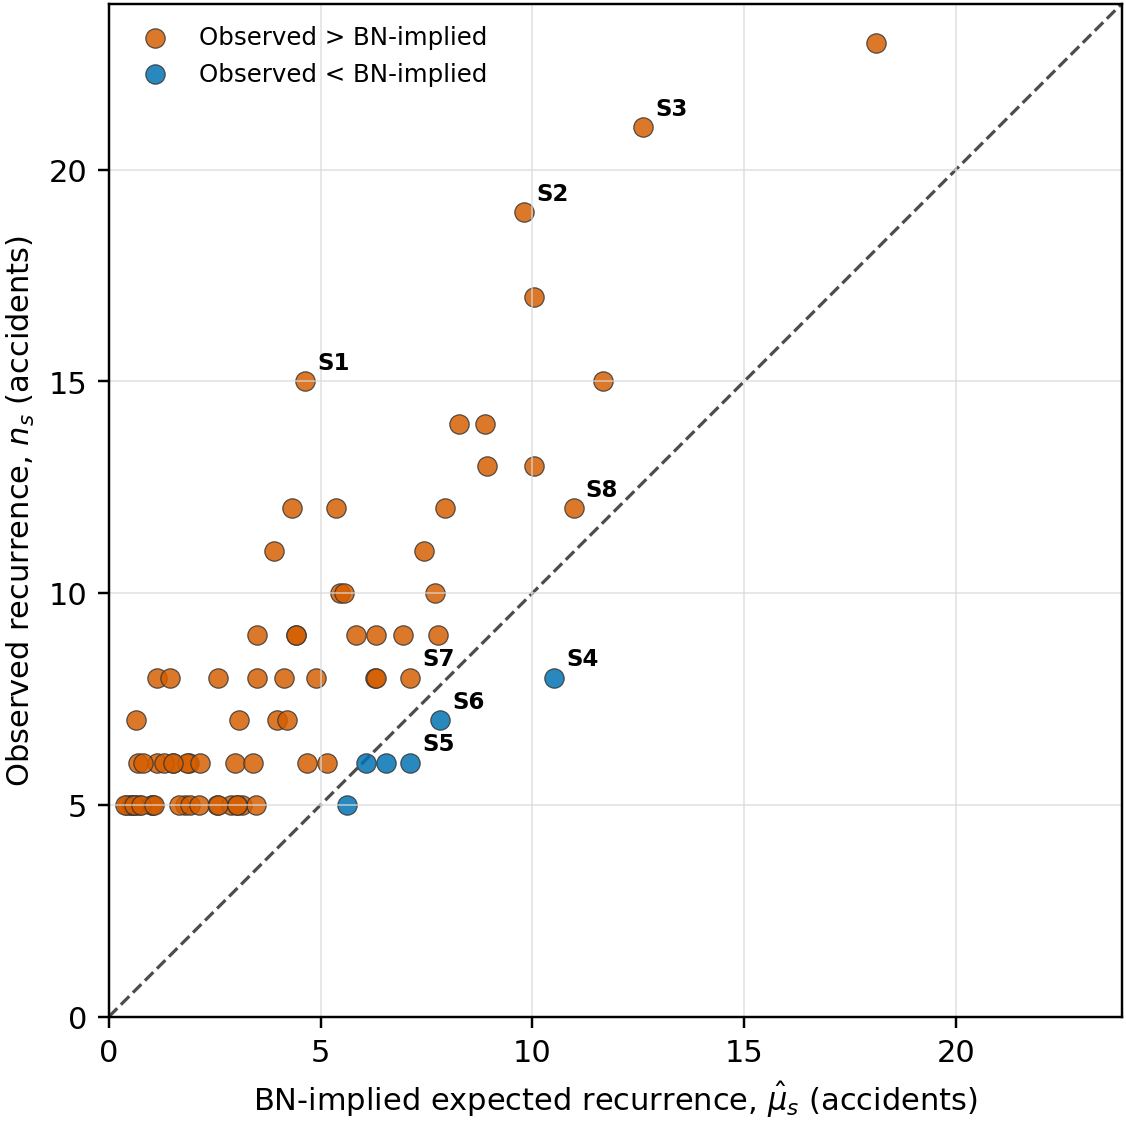
\includegraphics[
    width=0.82\textwidth
]{figs_ch4/observed_vs_bn_implied_recurrence_annotated.png}

\caption{
Observed versus BN-implied recurrence for recurrent closed scenarios
(\(n_{\min}=5\)). The dashed diagonal indicates exact agreement; labels refer
to Table~\ref{tab:chap4_carpentry_bn_recurrence}.
}
\label{fig:chap4_carpentry_bn_recurrence}
\end{figure}

\begin{table}[!htbp]
\centering
\scriptsize

\caption{Scenarios annotated in Figure~\ref{fig:chap4_carpentry_bn_recurrence}.
The difference is \(n_s-\widehat\mu_s\), in accidents.}
\label{tab:chap4_carpentry_bn_recurrence}

\renewcommand{\arraystretch}{1.08}
\setlength{\tabcolsep}{4pt}

\begin{tabularx}{\textwidth}{
    >{\centering\arraybackslash}p{0.06\textwidth}
    >{\raggedright\arraybackslash}X
    >{\centering\arraybackslash}p{0.09\textwidth}
    >{\centering\arraybackslash}p{0.13\textwidth}
    >{\centering\arraybackslash}p{0.12\textwidth}
}
\toprule
\textbf{ID} &
\textbf{Scenario} &
\shortstack{\textbf{Observed}\\\(n_s\)} &
\shortstack{\textbf{BN-implied}\\\(\widehat\mu_s\)} &
\shortstack{\textbf{Difference}\\\(n_s-\widehat\mu_s\)} \\
\midrule

S1 &
\shortstack[l]{(A0) Roof covering replacement and installation work\\
\(\rightarrow\) (B) Falls from elevated work areas\\
\(\rightarrow\) (C) Fatal outcomes after severe injuries} &
15 & 4.63 & \(+10.37\) \\

S2 &
\shortstack[l]{(A0) Roof work accessed by ladders\\
\(\rightarrow\) (B) Falls from elevated work areas\\
\(\rightarrow\) (C) Fatal traumatic injuries and multiple fractures} &
19 & 9.81 & \(+9.19\) \\

S3 &
\shortstack[l]{(A0) Construction structural assembly and temporary supports\\
\(\rightarrow\) (B) Falls from elevated work areas\\
\(\rightarrow\) (C) Fatal traumatic injuries and multiple fractures} &
21 & 12.61 & \(+8.39\) \\

S4 &
\shortstack[l]{(A0) Roof covering replacement and installation work\\
\(\rightarrow\) (B) Falls from elevated work areas\\
\(\rightarrow\) (C) Fatal traumatic injuries and multiple fractures} &
8 & 10.51 & \(-2.51\) \\

S5 &
\shortstack[l]{(A0) Construction carpentry and roofing work\\
\(\rightarrow\) (B) Falls from elevated work areas\\
\(\rightarrow\) (C) Multiple fractures across body regions} &
6 & 7.10 & \(-1.10\) \\

S6 &
\shortstack[l]{(A1) Missing or ineffective guards on cutting machinery\\
\(\rightarrow\) (B) Wood kickback drawing hands into rotating tools\\
\(\rightarrow\) (C) Finger and hand amputations} &
7 & 7.82 & \(-0.82\) \\

S7 &
\shortstack[l]{(A0) Short-term construction and repair operations\\
\(\rightarrow\) (B) Falls from elevated work areas\\
\(\rightarrow\) (C) Multiple fractures across body regions} &
8 & 7.10 & \(+0.90\) \\

S8 &
\shortstack[l]{(A0) Carpentry and building joinery work\\
\(\rightarrow\) (B) Falls from elevated work areas\\
\(\rightarrow\) (C) Fatal traumatic injuries and multiple fractures} &
12 & 10.97 & \(+1.03\) \\

\bottomrule
\end{tabularx}
\end{table}

The comparison shows both broad asymmetry and scenario-specific variation.
Seventy-four of the 80 recurrent scenarios lie above the equality line, while
six lie below it. The median absolute discrepancy is 3.96 accidents. The
largest positive discrepancies all concern fall configurations. These results
extend the preceding conditional-dependence analysis. In particular, the
presence of a fall--consequence dependency in the network does not require
the complete upstream--fall--consequence configuration to be reproduced at
its empirical frequency.

The scenarios close to the diagonal show the converse. The recurrence of S7
and S8 is well represented by the fitted joint distribution, whereas S4--S6
lie below the diagonal. Proximity to the diagonal is informative: it
identifies recurrent configurations that are compatible with the conditional
organization already represented by the network. It does not make them less
relevant as empirical accident scenarios.

This comparison provides information that is not captured by individual
network edges alone: a scenario may contain selected conditional dependencies
while its complete configuration is still reproduced poorly by the fitted
joint model.

These discrepancies are interpreted descriptively rather than as formal
goodness-of-fit tests. The same accident sample is used to estimate the
network and to identify recurrent scenarios, and the displayed scenarios have
already been selected according to an empirical recurrence threshold. The
predominance of positive discrepancies is consequently a feature of this
fitted, role-constrained network rather than a test result. Configurations
with large discrepancies provide focused targets for expert examination; they
do not by themselves establish model failure, an omitted causal mechanism, or
a prevention priority.

From a prevention perspective, this final comparison complements the previous
analyses. Scenario support identifies configurations that repeatedly occur,
the Bayesian network identifies direct conditional relationships among their
components, and the observed-versus-implied comparison indicates whether the
fitted probabilistic organization reproduces the recurrence of the complete
configuration. These quantities are therefore interpreted jointly but remain
conceptually distinct.

The complete inventory of the 80 recurrent closed configurations is reported
in Appendix~\ref{app:chap4_carpentry_scenarios_full}.
